
\begin{figure*}[ht]
% \label{fix:exp-results}
  \centering

  \begin{subfigure}[b]{0.45\textwidth}
    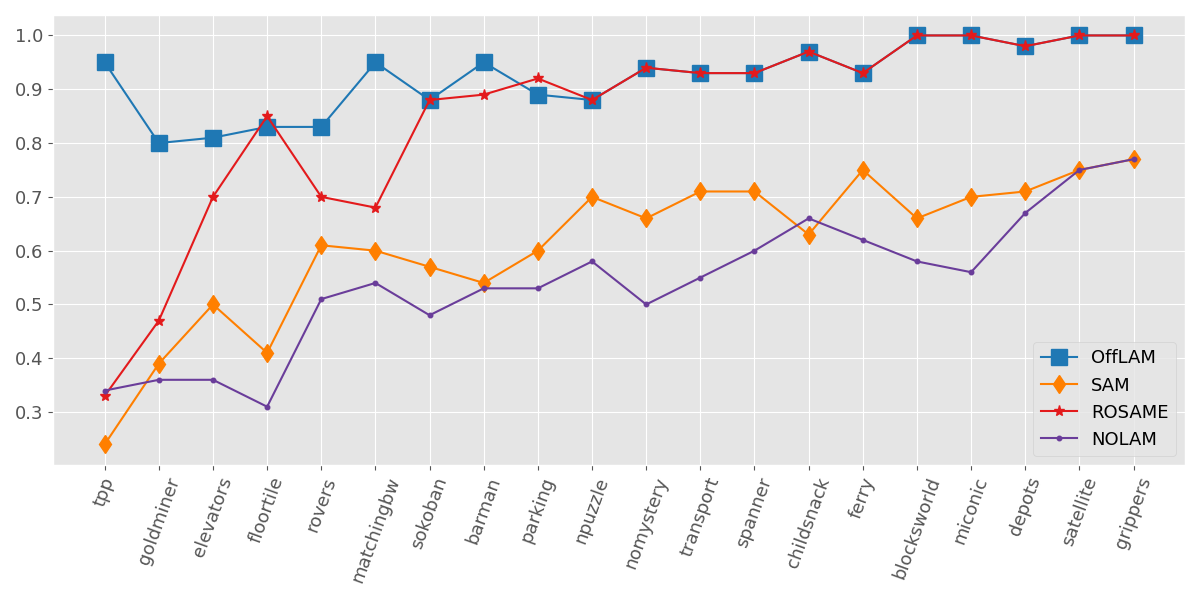
\includegraphics[width=\textwidth]{figures/10_traces/lineplots/syn_precision_line.png}
    \caption{Syntactic precision}
    \label{fig:syn-precision}
  \end{subfigure}
  % \hfill
  \begin{subfigure}[b]{0.45\textwidth}
    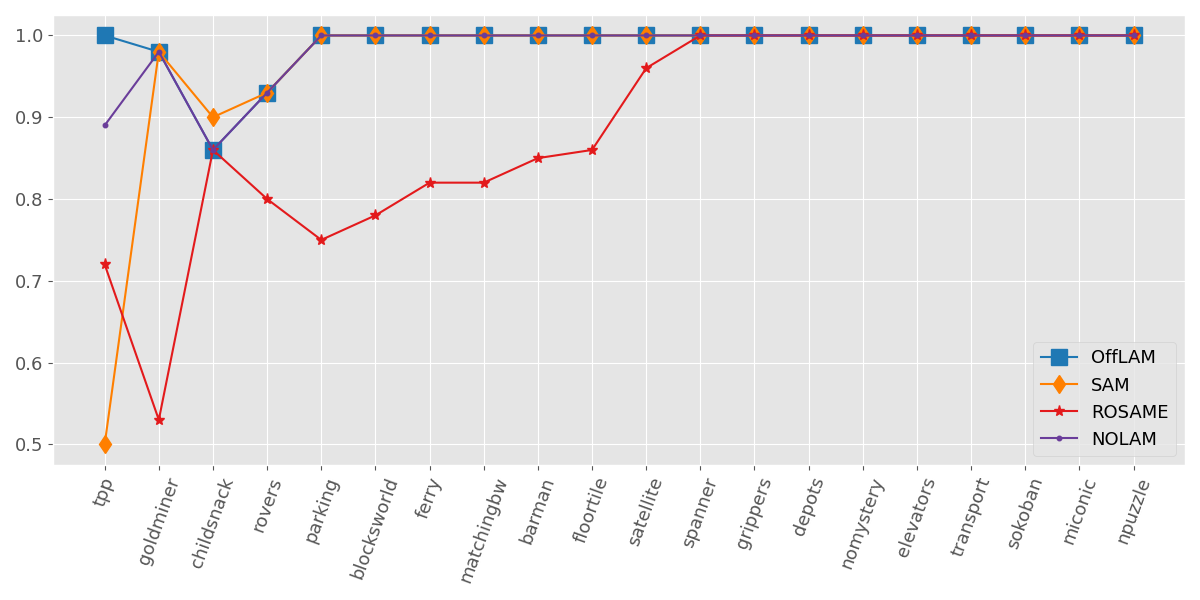
\includegraphics[width=\textwidth]{figures/10_traces/lineplots/syn_recall_line.png}
    \caption{Syntactic recall}
  \end{subfigure}

  \vspace{1em}

  \begin{subfigure}[b]{0.45\textwidth}
    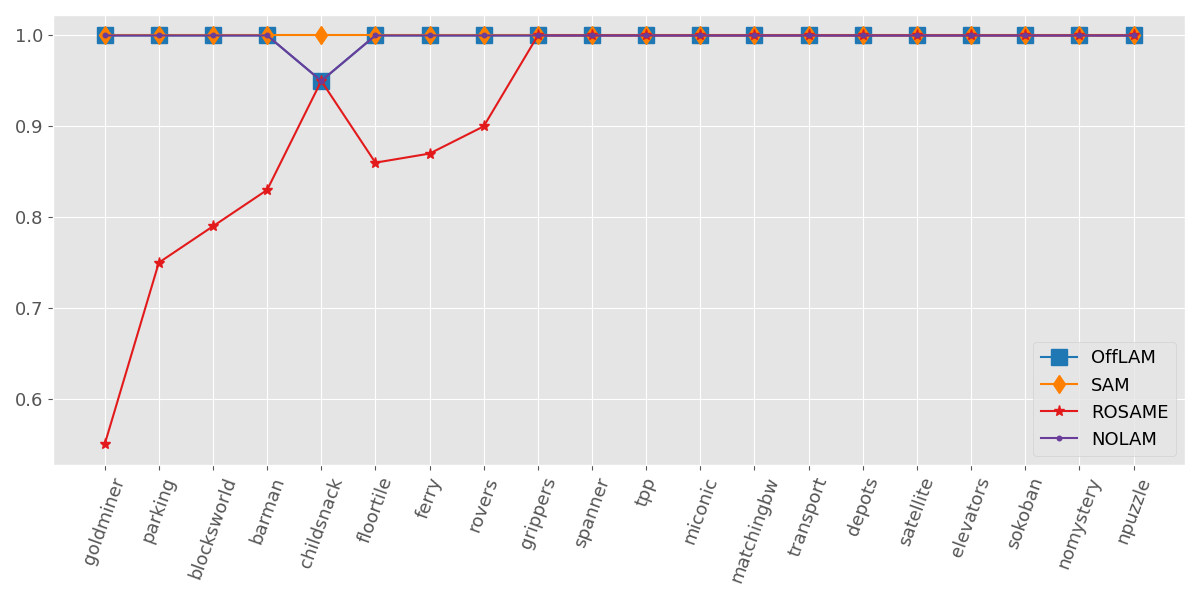
\includegraphics[width=\textwidth]{figures/10_traces/lineplots/app_precision_line.png}
    \caption{Applicability precision}
  \end{subfigure}
  % \hfill
  \begin{subfigure}[b]{0.45\textwidth}
    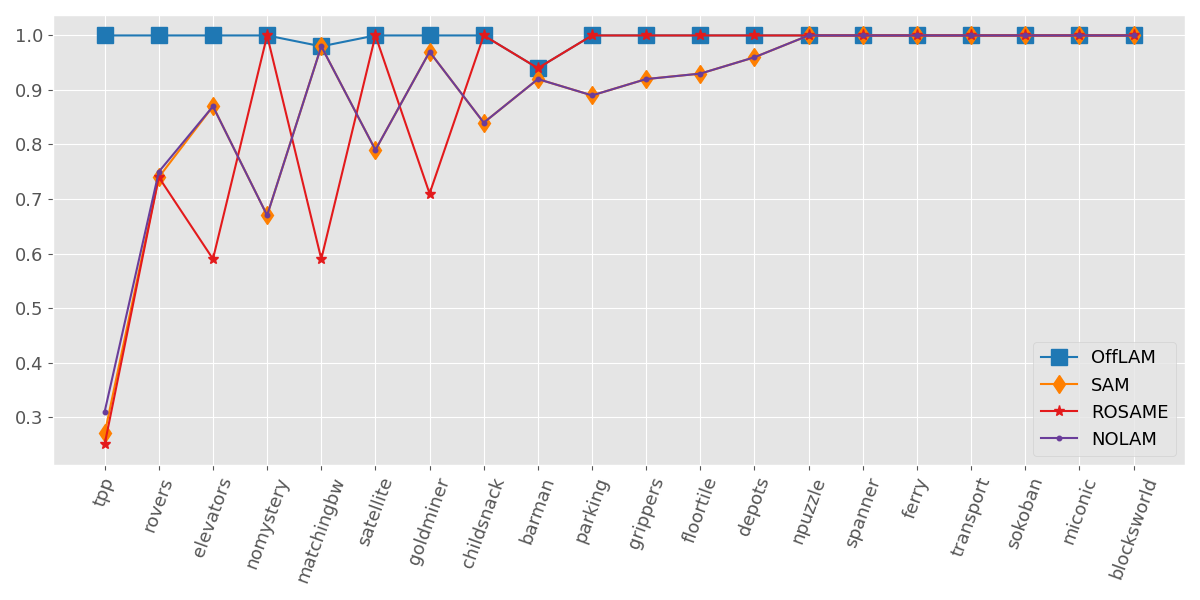
\includegraphics[width=\textwidth]{figures/10_traces/lineplots/app_recall_line.png}
    \caption{Applicability recall}
  \end{subfigure}

  \vspace{1em}

  \begin{subfigure}[b]{0.45\textwidth}
    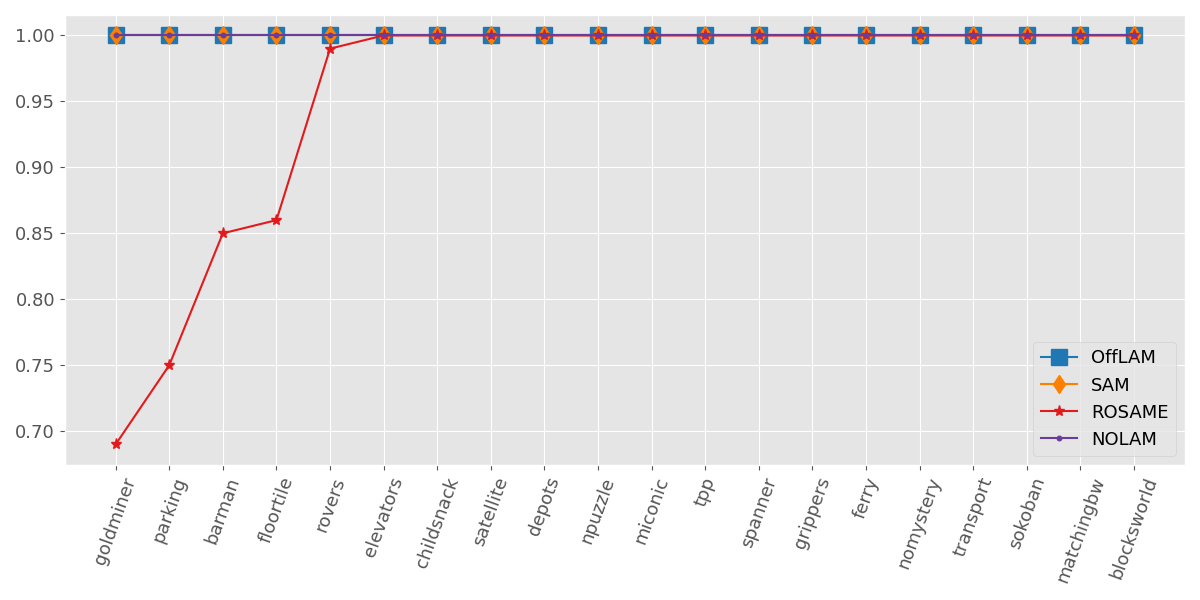
\includegraphics[width=\textwidth]{figures/10_traces/lineplots/predeffs_precision_line.png}
    \caption{Predicted effects precision}
  \end{subfigure}
  % \hfill
  \begin{subfigure}[b]{0.45\textwidth}
    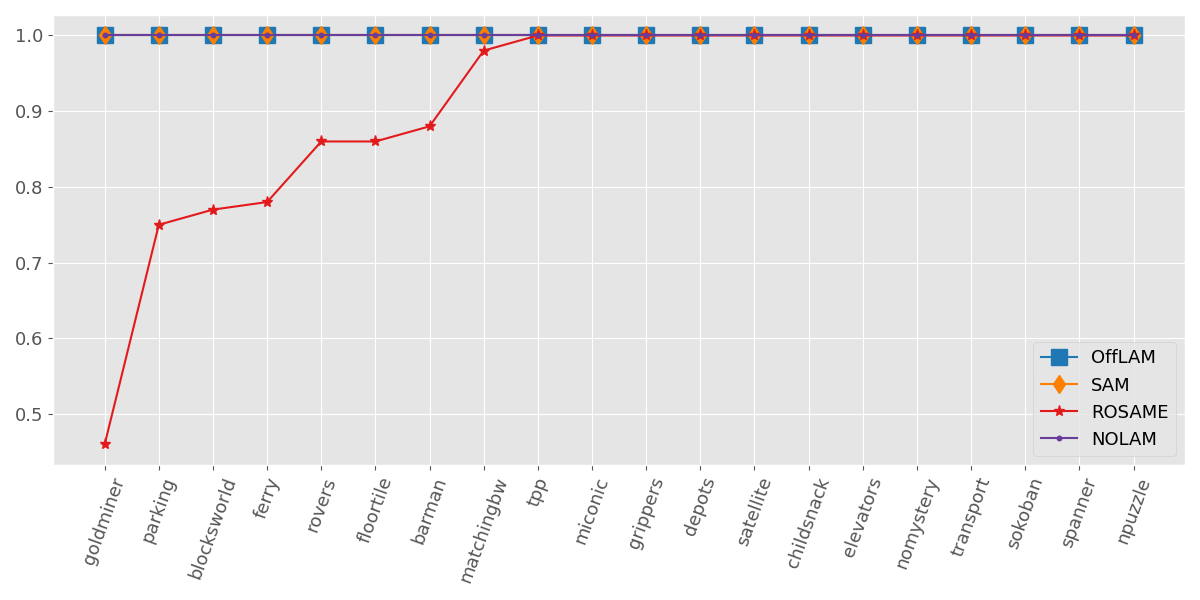
\includegraphics[width=\textwidth]{figures/10_traces/lineplots/predeffs_recall_line.png}
    \caption{Predicted effects recall}
  \end{subfigure}

  % \vspace{1em}

  % \begin{subfigure}[b]{0.45\textwidth}
  %   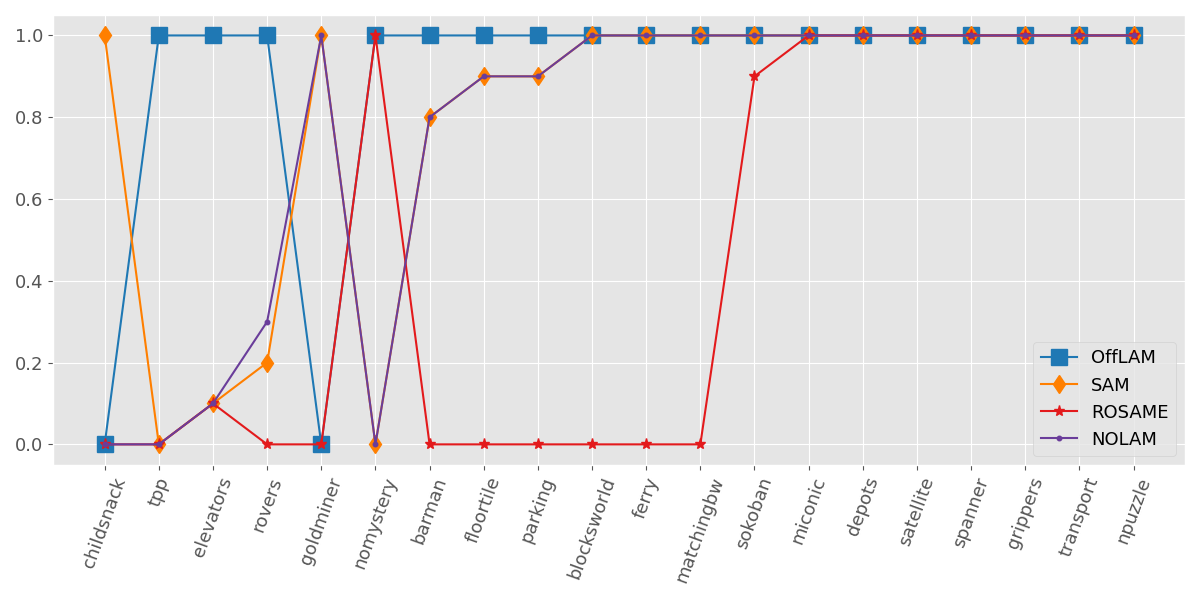
\includegraphics[width=\textwidth]{figures/10_traces/lineplots/solving_line.png}
  %   \caption{Problem solving ratio}
  %   \label{fig:solving-ratio}
  % \end{subfigure}
  % % \hfill
  % \begin{subfigure}[b]{0.45\textwidth}
  %   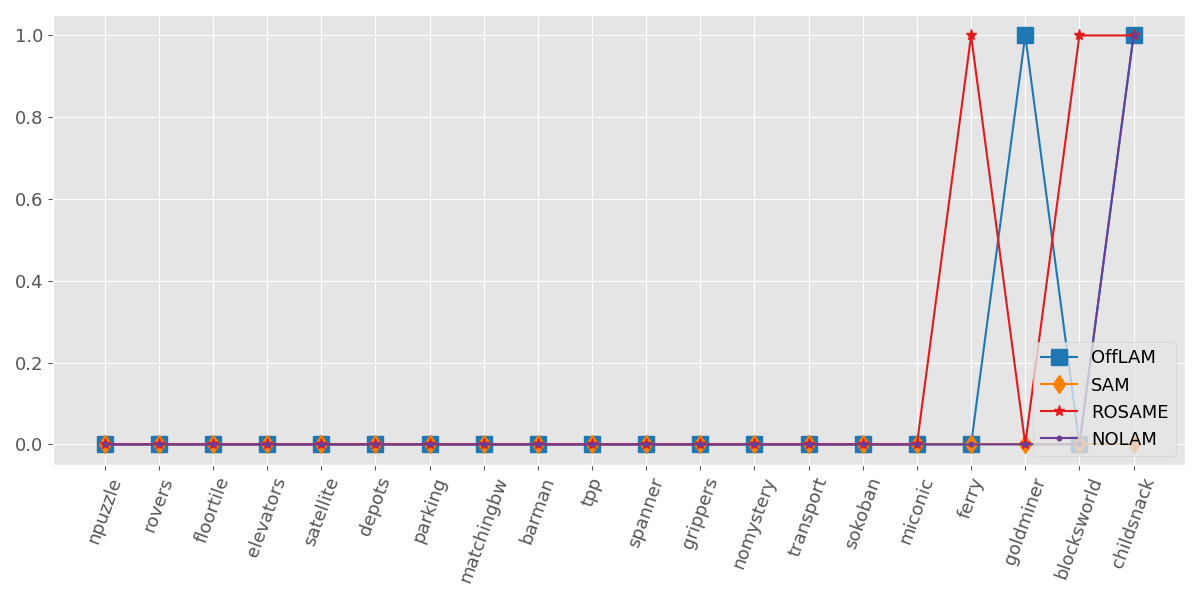
\includegraphics[width=\textwidth]{figures/10_traces/lineplots/false_plans_line.png}
  %   \caption{False plans ratio}
  %   \label{fig:false-positive-plans}
  % \end{subfigure}

  % \caption{Overall caption for the 6 images.}
  % \caption{Evaluation metrics when learning from a training set $\Ttrain$ with $10$ traces for every domain.}
\caption{Evaluation metric values for the models learned by \sam, \offlam, \nolam, and \rosame in every benchmark domain. The training set $\Ttrain$ includes $10$ trajectories for every domain. \roni{Not sure about these figures. Maybe the previous ones were better? } \leo{I re-added previous ones (i.e. barplots), after adding ROSAME results, the bar plots seem to me a bit overloaded}}
  % \label{fig:exp}
\end{figure*} 

\begin{table}[h]
\resizebox{\columnwidth}{!}{
\addtolength{\tabcolsep}{-0.4em}
\begin{tabular}{l|cccc|cccc|}
% \toprule
\hline
 & \multicolumn{4}{c|}{Solv. \% $\uparrow$} & \multicolumn{4}{c|}{False \% $\downarrow$} \\
Domain & \offlam & \samshort & \rosame & \nolam & \offlam & \samshort & \rosame & \nolam 
\\
% \midrule
\hline
barman & $\mathbf{1.00}$ & $0.80$ & $0.00$ & $0.80$ & $\mathbf{0.00}$ & $\mathbf{0.00}$ & $\mathbf{0.00}$ & $\mathbf{0.00}$ \\
blocksworld & $\mathbf{1.00}$ & $\mathbf{1.00}$ & $0.00$ & $\mathbf{1.00}$ & $\mathbf{0.00}$ & $\mathbf{0.00}$ & $1.00$ & $\mathbf{0.00}$ \\
childsnack & $0.00$ & $\mathbf{1.00}$ & $0.00$ & $0.00$ & $1.00$ & $\mathbf{0.00}$ & $1.00$ & $1.00$ \\
depots & $\mathbf{1.00}$ & $\mathbf{1.00}$ & $\mathbf{1.00}$ & $\mathbf{1.00}$ & $\mathbf{0.00}$ & $\mathbf{0.00}$ & $\mathbf{0.00}$ & $\mathbf{0.00}$ \\
elevators & $\mathbf{1.00}$ & $0.10$ & $0.10$ & $0.10$ & $\mathbf{0.00}$ & $\mathbf{0.00}$ & $\mathbf{0.00}$ & $\mathbf{0.00}$ \\
ferry & $\mathbf{1.00}$ & $\mathbf{1.00}$ & $0.00$ & $\mathbf{1.00}$ & $\mathbf{0.00}$ & $\mathbf{0.00}$ & $1.00$ & $\mathbf{0.00}$ \\
floortile & $\mathbf{1.00}$ & $0.90$ & $0.00$ & $0.90$ & $\mathbf{0.00}$ & $\mathbf{0.00}$ & $\mathbf{0.00}$ & $\mathbf{0.00}$ \\
goldminer & $0.00$ & $\mathbf{1.00}$ & $0.00$ & $\mathbf{1.00}$ & $1.00$ & $\mathbf{0.00}$ & $\mathbf{0.00}$ & $\mathbf{0.00}$ \\
grippers & $\mathbf{1.00}$ & $\mathbf{1.00}$ & $\mathbf{1.00}$ & $\mathbf{1.00}$ & $\mathbf{0.00}$ & $\mathbf{0.00}$ & $\mathbf{0.00}$ & $\mathbf{0.00}$ \\
matchingbw & $\mathbf{1.00}$ & $\mathbf{1.00}$ & $0.00$ & $\mathbf{1.00}$ & $\mathbf{0.00}$ & $\mathbf{0.00}$ & $\mathbf{0.00}$ & $\mathbf{0.00}$ \\
miconic & $\mathbf{1.00}$ & $\mathbf{1.00}$ & $\mathbf{1.00}$ & $\mathbf{1.00}$ & $\mathbf{0.00}$ & $\mathbf{0.00}$ & $\mathbf{0.00}$ & $\mathbf{0.00}$ \\
nomystery & $\mathbf{1.00}$ & $0.00$ & $\mathbf{1.00}$ & $0.00$ & $\mathbf{0.00}$ & $\mathbf{0.00}$ & $\mathbf{0.00}$ & $\mathbf{0.00}$ \\
npuzzle & $\mathbf{1.00}$ & $\mathbf{1.00}$ & $\mathbf{1.00}$ & $\mathbf{1.00}$ & $\mathbf{0.00}$ & $\mathbf{0.00}$ & $\mathbf{0.00}$ & $\mathbf{0.00}$ \\
parking & $\mathbf{1.00}$ & $0.90$ & $0.00$ & $0.90$ & $\mathbf{0.00}$ & $\mathbf{0.00}$ & $\mathbf{0.00}$ & $\mathbf{0.00}$ \\
rovers & $\mathbf{1.00}$ & $0.20$ & $0.00$ & $0.30$ & $\mathbf{0.00}$ & $\mathbf{0.00}$ & $\mathbf{0.00}$ & $\mathbf{0.00}$ \\
satellite & $\mathbf{1.00}$ & $\mathbf{1.00}$ & $\mathbf{1.00}$ & $\mathbf{1.00}$ & $\mathbf{0.00}$ & $\mathbf{0.00}$ & $\mathbf{0.00}$ & $\mathbf{0.00}$ \\
sokoban & $\mathbf{1.00}$ & $\mathbf{1.00}$ & $0.90$ & $\mathbf{1.00}$ & $\mathbf{0.00}$ & $\mathbf{0.00}$ & $\mathbf{0.00}$ & $\mathbf{0.00}$ \\
spanner & $\mathbf{1.00}$ & $\mathbf{1.00}$ & $\mathbf{1.00}$ & $\mathbf{1.00}$ & $\mathbf{0.00}$ & $\mathbf{0.00}$ & $\mathbf{0.00}$ & $\mathbf{0.00}$ \\
tpp & $\mathbf{1.00}$ & $0.00$ & $0.00$ & $0.00$ & $\mathbf{0.00}$ & $\mathbf{0.00}$ & $\mathbf{0.00}$ & $\mathbf{0.00}$ \\
transport & $\mathbf{1.00}$ & $\mathbf{1.00}$ & $\mathbf{1.00}$ & $\mathbf{1.00}$ & $\mathbf{0.00}$ & $\mathbf{0.00}$ & $\mathbf{0.00}$ & $\mathbf{0.00}$ \\
% \bottomrule
\hline
\end{tabular}
}
\caption{Problem solving (Solv.\%) and false plan ratio (False \%) achieved by planning with the domains learned by \offlam, \sam, \rosame, and \nolam; $\uparrow$ (resp. $\downarrow$) indicates the higher (resp. lower) the better, the best metric value for every domain is highlighted in bold.}
\label{tab:solving_ratio_false_plans_ratio}
\end{table}
